\hypertarget{earlyexiting}{%
	\chapter{Edge Offloading with Early Exiting}\label{ch:edgeoffloading}}
\thispagestyle{fancy}

In this chapter, section \ref{sec:edge-aee} presents our offloading scheme, section \ref{sec:edge-system-model} defines the system model, section \ref{sec:edge-implementation} describes our implementation, section \ref{sec:edge-results} presents our results, and lastly, section \ref{sec:edge-summary} summarizes our findings.

\section{\acrfull{aee} for Time-Critical Applications} \label{sec:edge-aee}

We propose \acrfull{aee}, an inference scheme based on an early exit \gls{dnn}. It utilizes the inherent properties of the early exit model. It adaptively maximizes the reliability using a best-effort approach by continuously returning predictions as they become ready. The inference is only terminated when a deadline is violated. The increasingly confident predictions from the continuous replies enable service not possible using conventional \gls{dnn}s. Our scheme is flexible as it can function for on-device, edge offloading, or collaborative inference architectures. 
\begin{figure}
	\captionsetup[subfigure]{justification=centering}
	\centering
	\subfloat[Continuous reply of predictions\label{fig:offloading-scheme-successful}]{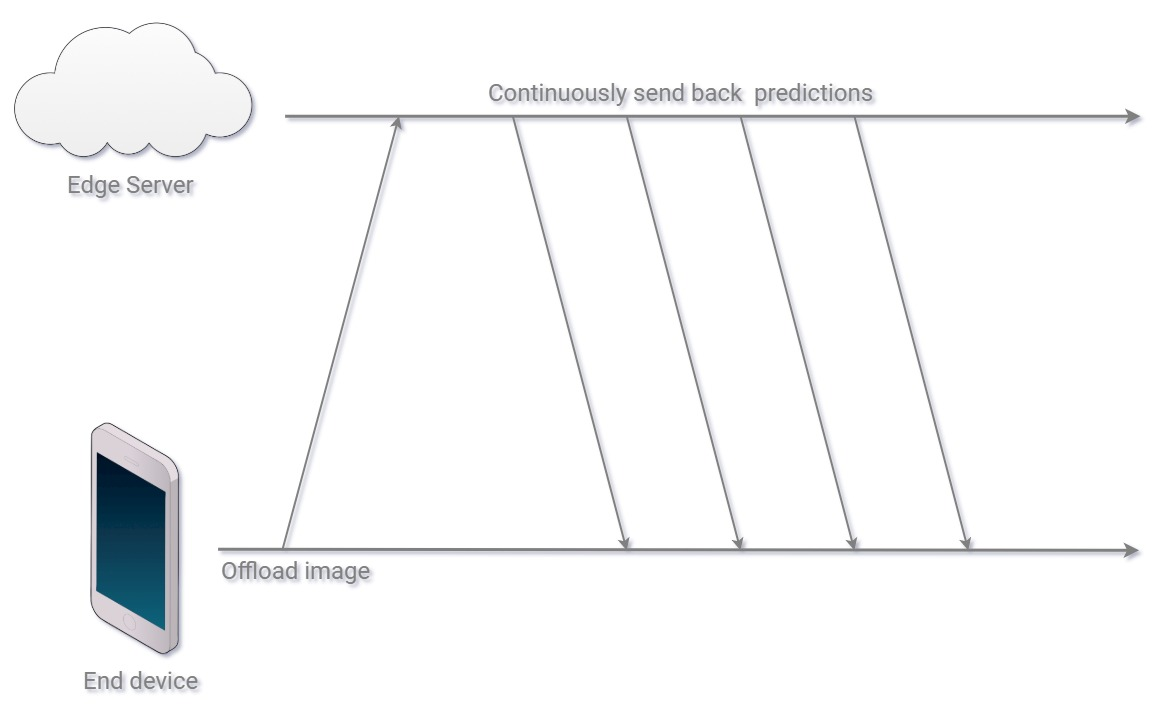
\includegraphics[width=.7\linewidth]{figures/models/timeline_all}}
\end{figure}
\begin{figure}
	\captionsetup[subfigure]{justification=centering}
	\centering
	\subfloat[Timeout interrupts the continuous reply of predictions\label{fig:offloading-scheme-timeout}]{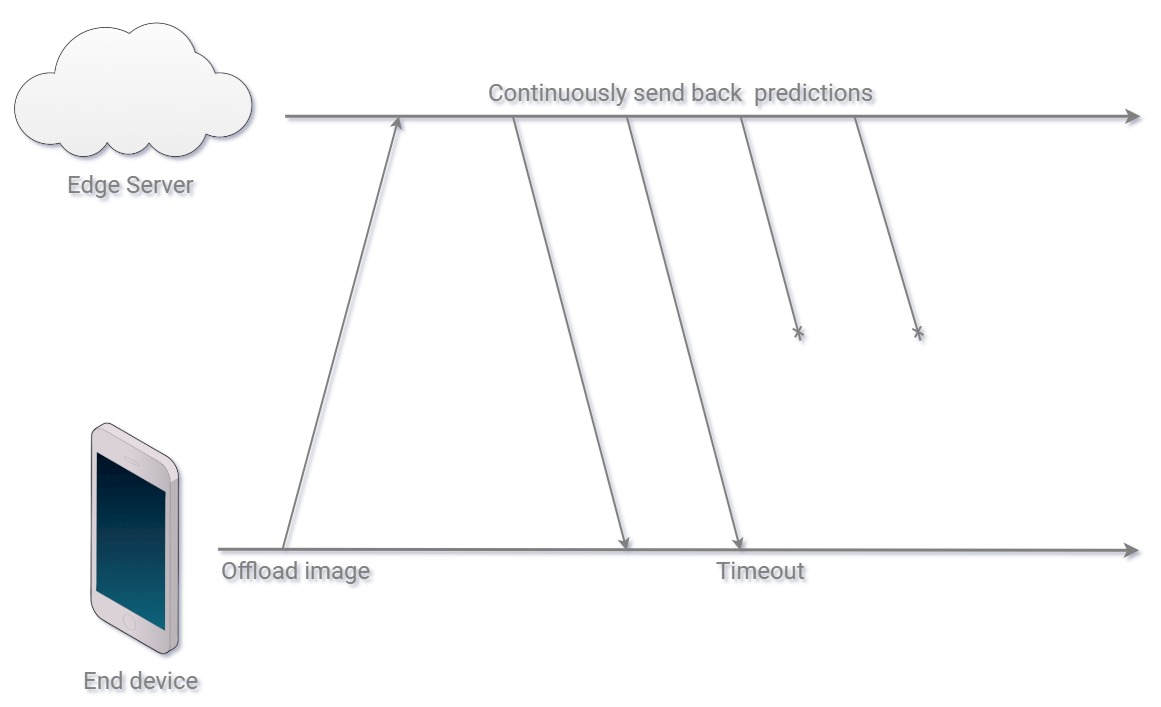
\includegraphics[width=.7\linewidth]{figures/models/timeline_timeout}}
	\caption[Offloading scheme]{\gls{aee} edge offloading: \protect\subref{fig:offloading-scheme-successful} continuous predictions received with no timeouts. \protect\subref{fig:offloading-scheme-timeout} Timeout interrupted the service, and only two predictions are available. }
	\label{fig:offloading-scheme}
\end{figure} 

Figure \ref{fig:offloading-scheme} illustrates the scheme in the context of edge offloading. Figure \ref{fig:offloading-scheme-successful} represents the continuous reply of predictions. Data is immediately offloaded upon acquisition from the end device to edge server not to waste idle time on the edge server. The edge server runs the inference process, and whenever a prediction is ready, it is sent back to the end device. Figure \ref{fig:offloading-scheme-timeout} illustrates a case where a timeout occurs. Timeouts occur when a deadline is violated. In this case, only two predictions are available. Timeouts can be caused by unexpected delays from congestions in the communication medium or due to high server workloads and others. Successively receiving prediction allow the user to select the prediction among the received replies. We examine ways to select the prediction using information from all responses.

\section{System Model} \label{sec:edge-system-model}
In this section, we define the system model for \gls{aee}. Note, the notations defined in chapter \ref{ch:earlyexit} is also used here, i.e., $ C $ denotes the number of the image classes, $ N $ denotes the number of the exit points in a DNN, $ I $ denotes the number of images. 	
\begin{enumdescript}
	\item[Latency]  We use $ T_{i,n}^{cmp} $ to denote computation time of inference, disregardless of the conventional model or the early exit model. 
	where the $ T_i^{cmp,loc} $, and $ T_i^{cmp,edge} $ are calculated following eq. \ref{eq:t_ci-and-t_ee}.
	We introduce two execution schemes; local processing and edge offloading.
	\begin{align}
	T_{i,n} = \begin{cases}
	T_{i,n}^{loc} \\
	T_{i,n}^{edge}
	\end{cases}
	\end{align}
	where $ T_{i,n}^{loc,cmp} $ denotes the computation time for local processing and $ T_{i,n}^{edge,cmp} $ denotes computation time at the edge. 
	Offloading for remote execution is only sensible whenever time can be saved over local execution, i.e.
	\begin{align*}
	T_{i,n}^{loc} > T_{i,n}^{edge}
	\end{align*}
	Due to the difference in computing resources, the compute time at the edge is expected to be significantly lower than local computation time, i.e., $ T_{i,n}^{loc,cmp} > T_{i,n}^{edge,cmp} $. 
	
	
	\begin{enumdescript}
		\item[Local Processing] Local runtime time is defined by the time to compute the inference
		\begin{align}
		T_{i}^{loc}= T_{i}^{cmp,loc}
		\end{align}
		\item[Edge Offloading] Edge offloading requires additional communication of data from local to remote and sending back results.
		\begin{align}
		T_{i}^{edge}=T_{i}^{com}+ T_{i}^{cmp,edge}
		\end{align}
		where $ T^{com}_i $ denotes the communication time, including the uplink time to transmit image $ i $ from local to edge, and the downlink time to send back reply to local. The communication time $ T^{com}_i $ becomes an important factor for offloading decisions, as the computing resources are expected to be more powerful on the edge servers.			
		
	\end{enumdescript}
	
	\item[Accuracy] Given the opportunity to receive multiple predictions within the time frame, it may be feasible to improve accuracy. Using the output results of the first $ n $ exit points to combine the information and select the most confident class. 
	\begin{align}
	\bar{A}^f &= 1 - \frac{1}{I} \sum_{i=1}^{I}\mathbb{I}\left(\left|\hat{c}_i^f-c_i\right|\right)
	\end{align}
	where the predicted class label $ \hat{c}_i^f = f(\bm{\hat{y}}_{i,1},\dots, \bm{\hat{y}}_{i,n}) $ is the output of the function that combines the score vector outputs from the available exit predictions. 
	
	There are several ways to define combination function $ f\left(\bm{\hat{y}}_{i,1}, \dots, \bm{\hat{y}}_{i,n}\right) $
	\begin{enumdescript}
		
		\item[Latest Recieved Prediction] assumes the last recieved prediction is the most confident as accuracy grows with exit depth. Thus, the method is constrained to only use the most recent prediction from exit $n$.
		\begin{align}
		f\left(\bm{\hat{y}}_{i,1}, \dots, \bm{\hat{y}}_{i,n} \right) = \hat{c}_{i,n}^{*}
		\end{align}
		
		\item[Max Confidence] assumes the highest scoring class among all available exits is the most confident prediction. The method is used in \cite{kaya_shallow-deep_nodate} and reports improvement on the \gls{cifar10}, \gls{cifar100}, and \gls{tinyimagenet}. 
		\begin{align}
		\begin{split}
		f\left(\bm{\hat{y}}_{i,1}, \cdots, \bm{\hat{y}}_{i,n} \right) =  \arg \underset{c}{\max} \{\hat{y}^*_{i,1}, ..., \hat{y}^*_{i,C} \},
		\\ \text{where\:} \hat{y}^*_{i,c} = \max \{\hat{y}_{i,1,c}, ..., \hat{y}_{i,n,c}\}
		\end{split}	
		\end{align}
		\item[Sum Confidence] assumes the collective knowledge from all exits can be used to find the prediction that the available exits agree upon by summing the scores for the class. The class with the highest score becomes the prediction.
		\begin{align}
		\begin{split}
		f\left(\bm{\hat{y}}_{i,1}, \dots, \bm{\hat{y}}_{i,n} \right) = \arg \underset{c}{\max} \{s_{i,1}, \dots, s_{i,C}\}, \\ \text{where\:} s_{i,c} = \sum_{j=1}^{n}\hat{y}_{i,n,c}\: \forall \ 1\le c \le C
		\end{split}
		\end{align}			
		\item[Max Score-Margin] assumes the class with the largest score-margin among all available exits is the most confident prediction. 			\begin{align}
		\begin{split}
		f\left(\bm{\hat{y}}_{i,1}, \dots, \bm{\hat{y}}_{i,n} \right) =c^*_{1,\hat{n}},\\
		\text{where\:} \hat{n} \in \{1, 2, ..., n\}
		\end{split}	
		\end{align}
		this means $ \hat{n} $ is the exit that provided the prediction with the largest score-margin, i.e.
		\begin{align*}
		\begin{split}
		\hat{n} = \arg \underset{j}{\max} \left\{f_{margin}(\bm{y}_{i,1}), ..., f_{margin}(\bm{y}_{i,n})\right\} ,\\
		\text{where\:} j \text{\:is an integer and\:} 1 \le j \le n
		\end{split}
		\end{align*}
		Note, $ f_{margin} $ is defined in eq. \ref{eq:f_margin}.
	\end{enumdescript}
	
	\item[Reliability]  Our primary concern is still time-critical applications. The redefined accuracy that uses the combination function is now used to redefine reliability as the obtainable accuracy before the deadline $ \delta $.
	
	\begin{align}
	R^f= \bar{A^f} \cdot (1-\overline{F}^{to})
	\end{align}
	
	The timeout probability $ \overline{F}^{to} $ is also still defined as the number of samples not able to meet the delay requirement out of all samples in the set. However, our latency is now not only dependent on computation time, but also communication time when offloading.
	\begin{align}
	\overline{F}^{to}=\frac{1}{I}\sum_{i=1}^{I} \mathbb{I}\left(T_{i}-\delta\right)
	\end{align}
	Where the inference latency is either local or edge offloading i.e.
	\begin{align*}
	T_{i} = \begin{cases}
	T_{i}^{loc} \\
	T_{i}^{edge}
	\end{cases}
	\end{align*}
	We have a delay violation if no prediction is provided before the deadline, i.e., $ T_{i} > \delta $  
	
	\item[Problem] As in chapter \ref{ch:earlyexit}, we define a maximization problem. The aim is to maximize the reliability for each image by selecting the best possible exit
	\begin{maxi}
		{\bm{n}}{\bar{R}^f}
		{}{}
		%\addConstraint{T_{i,n}}{\leq \delta}
	\end{maxi}
	where $ \bm{n} = \left\{ n_1, n_2, \dots, n_I \right\}$ is a vector to denote which exit point would be used for prediction image $ i $ from available exit point $ n_i \in \left\{1,2, \dots, N\right\} $.
	
	Similar to chapter \ref{ch:earlyexit}, we solve this problem by the best-effort scheme, i.e., feed each exit results back and let the user decide the prediction. We argue for best-effort over upfront exit decision for the following reasons:
	\begin{enumerate}
		\item latency uncertainty, not least from newly introduced communication, makes it hard to make an exit decision in advance
		\item delay overhead from algorithm to make the decision is comparable with the delay overhead from the classifier of each exit point \cite{li_edge_2018}
	\end{enumerate}
	
	
\end{enumdescript}  

\section{Implementation} \label{sec:edge-implementation}

The offloading scheme is implemented as a client/server application \cite{sommerville_software_2015}, illustrated by the sequence diagram in figure \ref{fig:sequence-diagram}. 

\begin{figure}
	\captionsetup[subfigure]{justification=centering}
	\centering
	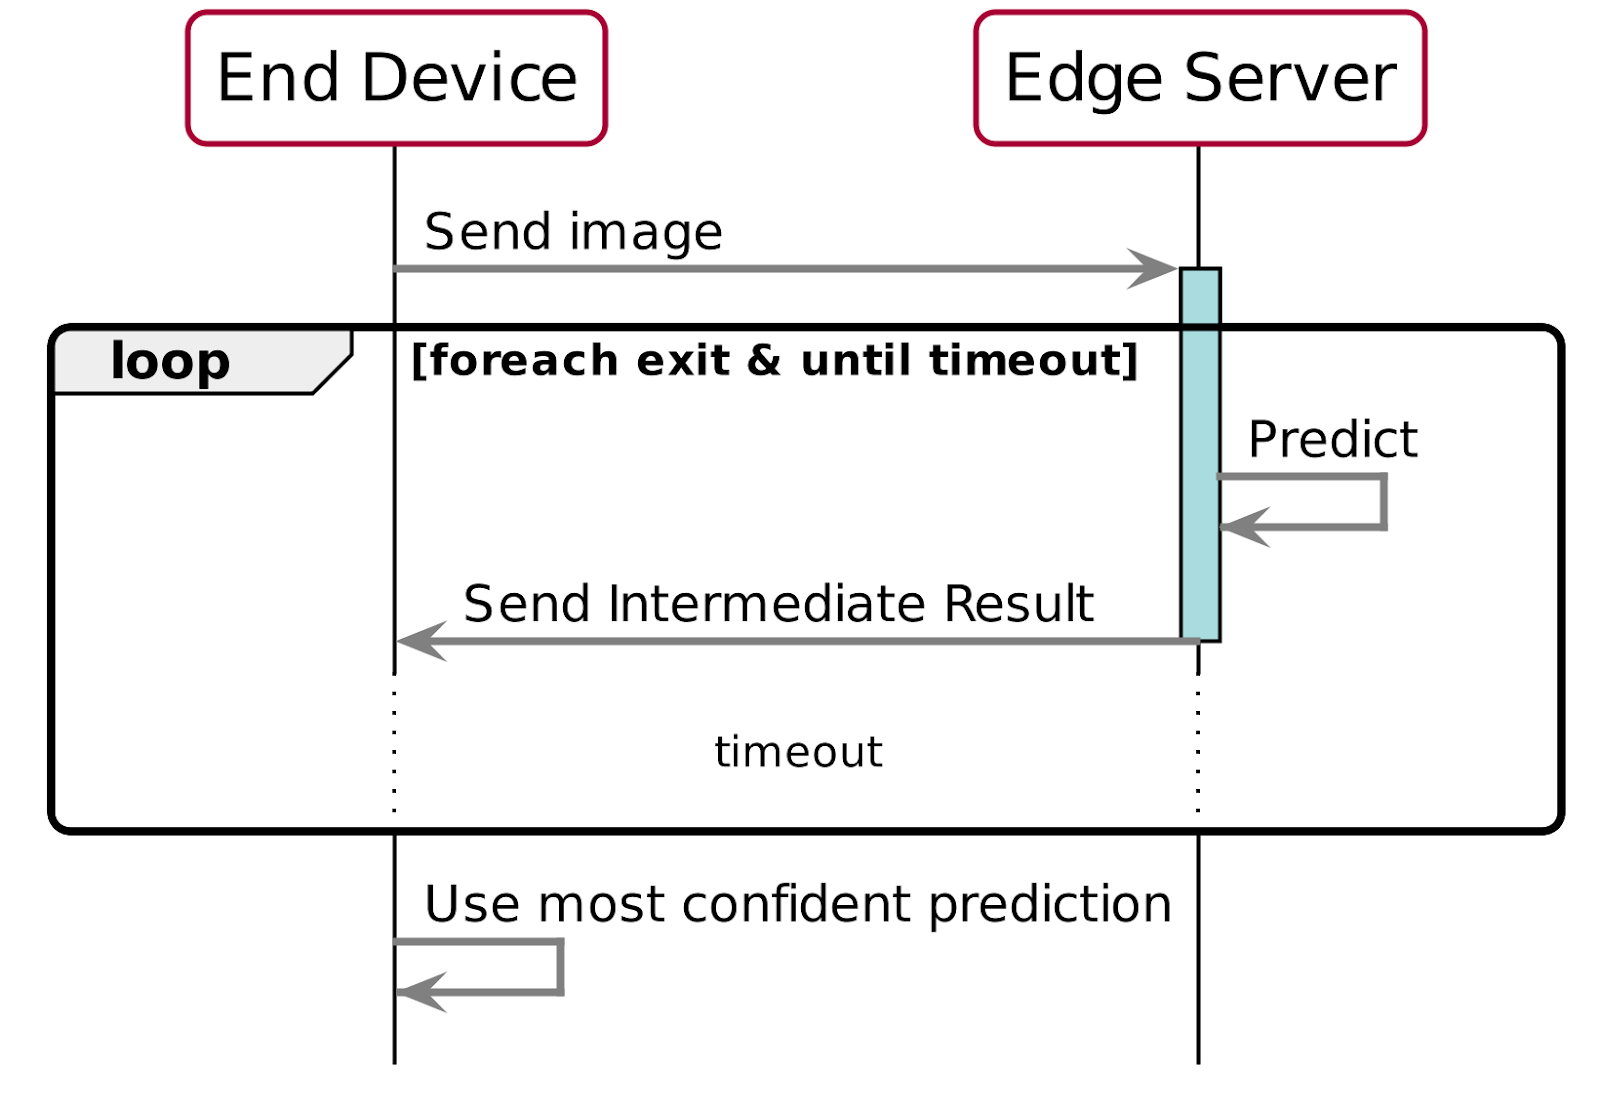
\includegraphics[width=.7\linewidth]{figures/models/sequence_diagram}
	\caption[Sequence Diagram \acrshort{aee}]{Sequence Diagram \acrshort{aee}: The client and server establish a TCP socket connection. The client loads a sample from the \gls{min100} validation set and streams the sample to the server. The server runs the model inference, and as soon as prediction is ready, a thread is spawned to stream the results back to the end device.}
	\label{fig:sequence-diagram}
\end{figure}

The implementation is written in \gls{python} using the \gls{python} Socket API \cite{noauthor_socket_nodate}, \gls{pytorch} \cite{paszke_automatic_2017}, and \gls{torchvision} \cite{marcel_torchvision_2010}. The client is deployed on the \gls{nuc} and the server on \gls{jetson} and \gls{gpu-ws}. The servers are LAN connected to the router, and the client is connected over the WLAN.

\paragraph{Information Combination}

Given the fact that the correct class is within these five predictions close to 90 \% of the time having just two predictions available for any of the models see figure \ref{fig:top-5-cumulative}. We limit the application to send back the top-5 class predictions to reduce the size of the reply and still be able to combine information. 

Each exit outputs two 5-dimensional vectors. $\bm{\hat{c}}_{i,k}^{top5}$ contains the labels of the top-5 classes, and $ \bm{\hat{y}}_{i,k}^{top5}$ includes the scores for the top-5 classes. To be able to combine information from $ n $ exits, we must expand the vectors back to the original class space of $ C $ dimensions.

\begin{align}
\begin{split}
\bm{\hat{c}}_{i,n}^{top5} &= \begin{bmatrix}
\hat{c}_{i,n}^{1st} & \phantom{.}\hat{c}_{i,n}^{2nd} & \phantom{.}\hat{c}_{i,n}^{3rd} & \phantom{.}\hat{c}_{i,n}^{4th} & \phantom{.}\hat{c}_{i,n}^{5th}
\end{bmatrix}, \\
\bm{\hat{y}}^{top5}_{i,n} &= \begin{bmatrix}
\hat{y}_{i,n}^{1st} & \phantom{.}\hat{y}_{i,n}^{2nd} & \phantom{.}\hat{y}_{i,n}^{3rd} & \hat{y}_{i,n}^{4th} & \phantom{.}\hat{y}_{i,n}^{5th}
\end{bmatrix}
\end{split}
\end{align}

The vectors are sorted from highest to lowest; hence the score $ \hat{y}_{i,k}^{1st} $ is associated with the class label $ c_{i,k}^{1st} $, and so on. 
We define an expansion function 
\begin{align}
f_{expand}\left(\bm{\hat{y}}_{i,n}^{top5},\bm{\hat{c}}_{i,n}^{top5}\right) = 
\begin{bmatrix}
\hat{y}_{i,n,1} & \hat{y}_{i,n,2} & \hat{y}_{i,n,c} & \dots & \hat{y}_{i,n,C}
\end{bmatrix}_{1 \times C}
\end{align}
The function takes as input the top-5 score vector $ \bm{\hat{y}}_{i,n}^{top5}$ and top-5 class label vector  $\bm{\hat{c}}_{i,n}^{top5}$. The function outputs a $ C $-dimensional score vector with scores at indices corresponding to the class label. 

\subparagraph{Example: Expansion of a 10 class problem} 
\blockquote[]{	 	
	For this $C=10$ example, we receive two output vectors $\bm{\hat{c}}_{i,n}^{top5}$ and $ \bm{\hat{y}}_{i,n}^{top5}$.
	\begin{align*}
	\bm{\hat{c}}_{i,n}^{top5} &= \begin{bmatrix}
	\phantom{0}0\phantom{.0} & \phantom{0}3\phantom{.0} & \phantom{0}6\phantom{.0} & \phantom{0}8\phantom{.0} & \phantom{0}9\phantom{.0}
	\end{bmatrix},\\
	\bm{\hat{y}}_{i,n}^{top5} &= \begin{bmatrix}
	0.80 & 0.10 & 0.05 & 0.03 & 0.01
	\end{bmatrix}
	\end{align*}
	We use our expansion function $ f_{expand}\left(\bm{\hat{y}}_{i,n}^{top5},\bm{\hat{c}}_{i,n}^{top5}\right) $, which return the score vector $ \mathbf{\hat{y}}_{i,n}$, for the respective classes in $ \bm{c}_{i,n} $
	\begin{align*}
	\mathbf{\hat{y}}_{i,n}  &= \begin{bmatrix}
	0.80 & 0.00 & 0.00 & 0.10 & 0.00 & 0.00 & 0.05 & 0.00 & 0.03 & 0.01
	\end{bmatrix}_{1 \times 10} \\
	\bm{c}_{i,n} &= \begin{bmatrix}
	\phantom{0}0\phantom{.0} & \phantom{0}1\phantom{.0} & \phantom{0}2\phantom{.0} & \phantom{0}3\phantom{.0} & \phantom{0}4\phantom{.0} & \phantom{0}5\phantom{.0} & \phantom{0}6\phantom{.0} & \phantom{0}7\phantom{.0} & \phantom{0}8\phantom{.0} & \phantom{0}9\phantom{.0}
	\end{bmatrix}_{1 \times 10},
	\end{align*}
}      

Having multiple score vectors $ \left\{\bm{\hat{y}}_{i,1}, \dots, \bm{\hat{y}}_{i,n}\right\}  $ in the original class space allows us to formulate a $ n \times C $ score matrix, $ \bm{\hat{Y}}_{i}^{n \times C} $.
\begin{align}
\bm{\hat{Y}}_{i}^{n \times C} =
\begin{bmatrix}
\hat{y}_{i,1,1} & \hat{y}_{i,1,2} & \dots & \hat{y}_{i,1,C} \\
\hat{y}_{i,2,1} & \hat{y}_{i,,2} & \dots & \hat{y}_{i,2,C} \\
\vdots & \vdots & \ddots & \vdots \\
\hat{y}_{i,n,1} & \hat{y}_{i,n,2} & \dots & \hat{y}_{i,n,C}
\end{bmatrix}
\end{align}

Formulating as matrix ease the implementation of combination functions using \gls{numpy} \cite{oliphant_numpy:_2006}. 
\subparagraph{Example: Prediction matrix and information combination} 
\blockquote[]{	 	
	For this classification example, the number of classes $C=10$. We receive three predictions within a time frame and assume the predictions have been expanded.
	
	We construct the matrix $ \bm{\hat{Y}}_{i}^{n \times C} $
	\begin{align*}
	\bm{\hat{Y}}_{i}^{n \times C} =
	\begin{bmatrix}
	0.80 & 0.00 & 0.00 & 0.10 & 0.00 & 0.00 & 0.05 & 0.00 & 0.03 & 0.01 \\
	0.10 & 0.00 & 0.00 & 0.01 & 0.00 & 0.85 & 0.00 & 0.02 & 0.00 & 0.02 \\
	0.15 & 0.00 & 0.00 & 0.02 & 0.01 & 0.00 & 0.00 & 0.80 & 0.00 & 0.02 
	\end{bmatrix}_{3 \times 10}
	\end{align*}
	Using the defined combination functions yields the following results:
	\begin{enumerate}
		\item Using the method latest received prediction, the resulting prediction becomes label 7.
		\item Using the method maximum confidence, the resulting prediction becomes label 5.
		\item Using the method sum confidence, we sum all columns to create a new score vector
		\begin{align*}
		\bm{\hat{y}^{**}_{i}} = 
		\begin{bmatrix}
		1.05 & 0.00 & 0.00 & 0.13 & 0.01 & 0.85 & 0.05 & 0.82 & 0.03 & 0.05
		\end{bmatrix}_{1 \times 10}
		\end{align*}
		The resulting prediction becomes label 0.
		\item Using the method max score-margin, we find the largest difference between the two highest scores. The largest difference is found in the second row. Thus, the resulting prediction becomes label 5.
	\end{enumerate}
	Combining the scores gives different outcomes for the combination functions in this theoretical yet realistic example.
	
}

\section{Results} \label{sec:edge-results}

In this section, we present an academic study of using the combination functions. We have conducted practical experiments to maximize the reliability when offloading the inference task to the edge using both the early exit models and the conventional models. We compare local processing on the \gls{nuc} as end-device and edge offloading to \gls{jetson} or \gls{gpu-ws} as edge servers, and we evaluate the impact of reliable communication when offloading using \gls{tcp}. 

\subsection{Information Combination Analysis}

We examine the possibility of combining information from multiple predictions to improve accuracy. We studied top-1 prediction results and found that we encounter overthinking as in \cite{kaya_shallow-deep_nodate}. A concrete example is the 6th sample from the \gls{bresnet}.
\begin{align*}
c_6=0,
\bm{\hat{c}}_{6}=
\begin{bmatrix}
0 \\
54 \\
62 \\
62
\end{bmatrix},
\bm{\hat{y}}^{*}_{6}=
\begin{bmatrix}
0.56 \\
0.32 \\
0.52 \\
0.62
\end{bmatrix} \text{\:and\:}
\bm{b}_{6}=
\begin{bmatrix}
1 \\
0 \\
0 \\
0
\end{bmatrix}
\end{align*}
Where $ c_6 $ is the ground truth class label, $ \bm{\hat{c}}_6 $ is the predicted class labels from exit 1-4, $ \hat{y}^*_6 $ is the corresponding prediction score for the class label at all exits. $ b $ denotes the correctness of each exit as a binary value, where 1 is correct 0 is incorrect.

The prediction from the first exit is correct. However, based on the scores, the model is more confident about the last prediction. The predicted class becomes 62, using max confidence to determine the prediction. In \cite{kaya_shallow-deep_nodate}, they show marginal improvements using max confidence. Unfortunately, we did not achieve the same improvements. Table \ref{tbl:latest-vs-max} shows the accuracy of the models when having a prediction from all exits available.
	\begin{longtabu}{>{\bfseries}X|X|X}
		\caption[Lastest Received Prediction vs. Max score using Top-1]{Lastest Received Prediction vs. Max score using Top-1} \label{tbl:latest-vs-max} \\
		\toprule
		\rowfont{\bfseries}
		Model & Latest Received Prediction & Max Score   \tabularnewline
		\bottomrule
		\endfirsthead
		\multicolumn{3}{@{}l}{\textbf{\textcolor{black}{Table \ref{}:}} continued}\\
		\toprule
		\rowfont{\bfseries}
		Model & $Exit_N$ & max score    \tabularnewline
		\bottomrule
		\endhead % all the lines above this will be repeated on every page
		\bottomrule
		\multicolumn{3}{@{}l}{continued \ldots}\\
		\endfoot
		\hline
		\endlastfoot
		B-Resnet	& 0.8826	& 0.8794  \tabularnewline
		\hline
		B-DenseNet	& 0.8660 	& 0.8602 \tabularnewline
		\hline
		MSDNet		& 0.8640 	& 0.8598 \tabularnewline							
		\bottomrule
	\end{longtabu}

Using the confidence max reduces the accuracy compared to the latest received prediction. The small reduction using max confidence is most likely caused by more significant uncertainties from the less accurate early exits. In \cite{kaya_shallow-deep_nodate}, they do not operate with a time constraint and always have all predictions available. We cannot be sure to have received all predictions within the time frame. Our goal is to improve accuracy when all predictions are not available. 
\begin{figure}
	\captionsetup[subfigure]{justification=centering}
	\centering
	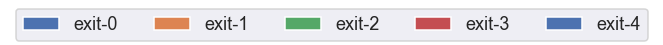
\includegraphics[width=.7\linewidth]{figures/edge/exit0-4_legend}
	\subfloat[B-ResNet\label{fig:exit-highscore-resnet}]{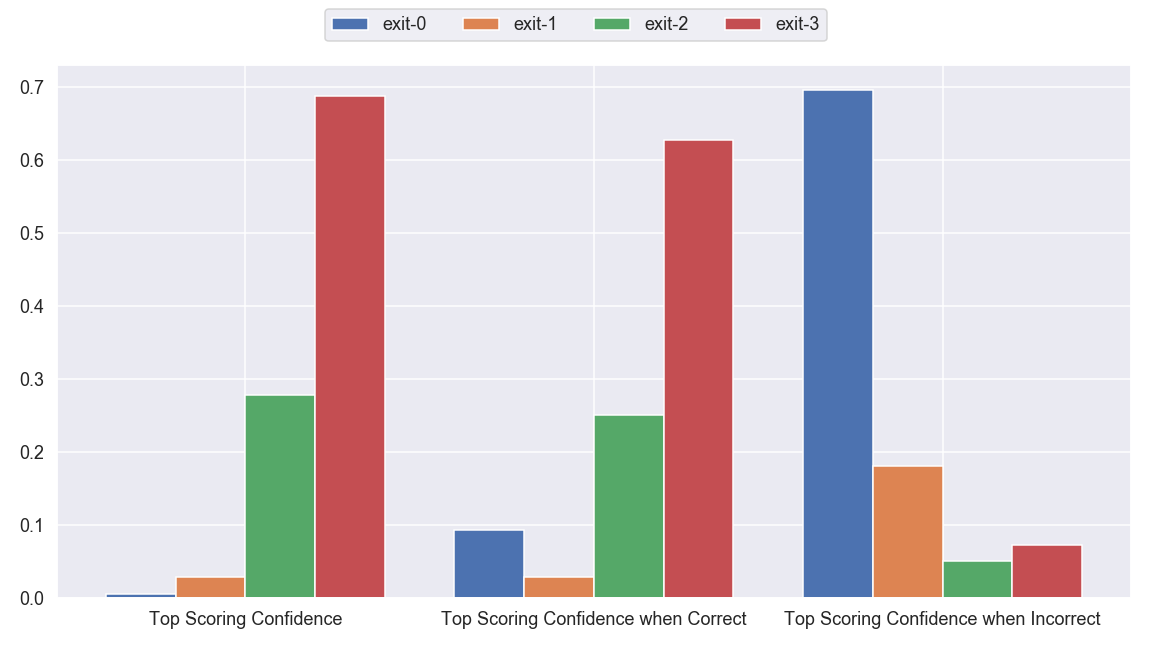
\includegraphics[width=.33\linewidth]{figures/edge/b-resnet_correctness}}
	\hfill
	\subfloat[B-DenseNet\label{fig:exit-highscore-densenet}]{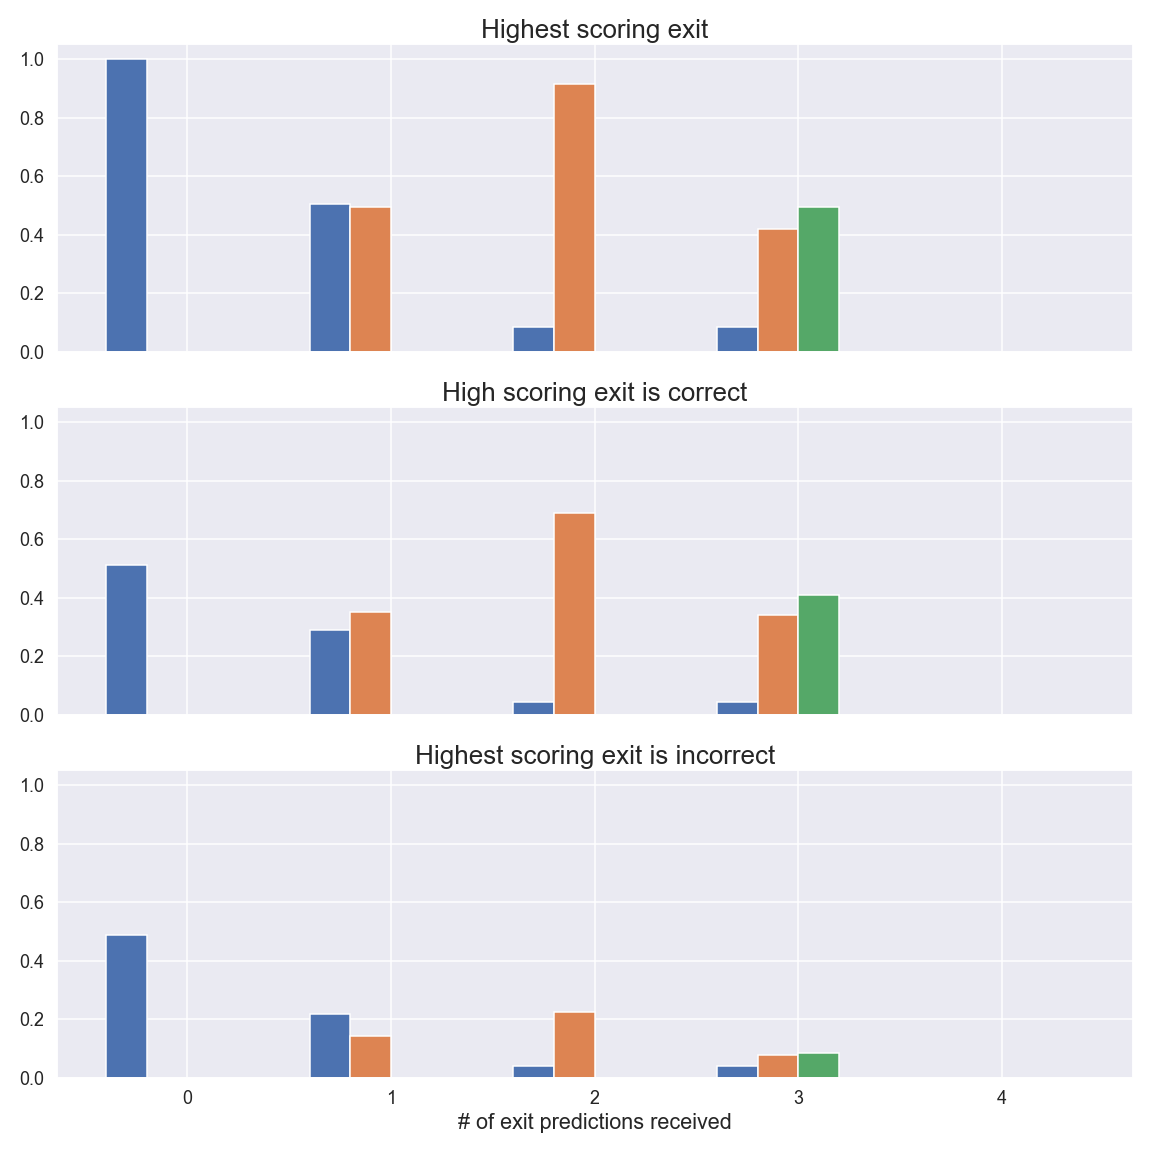
\includegraphics[width=.33\linewidth]{figures/edge/b-densenet_correctness}}
	\hfill
	\subfloat[MSDNet\label{fig:exit-highscore-msdnet}]{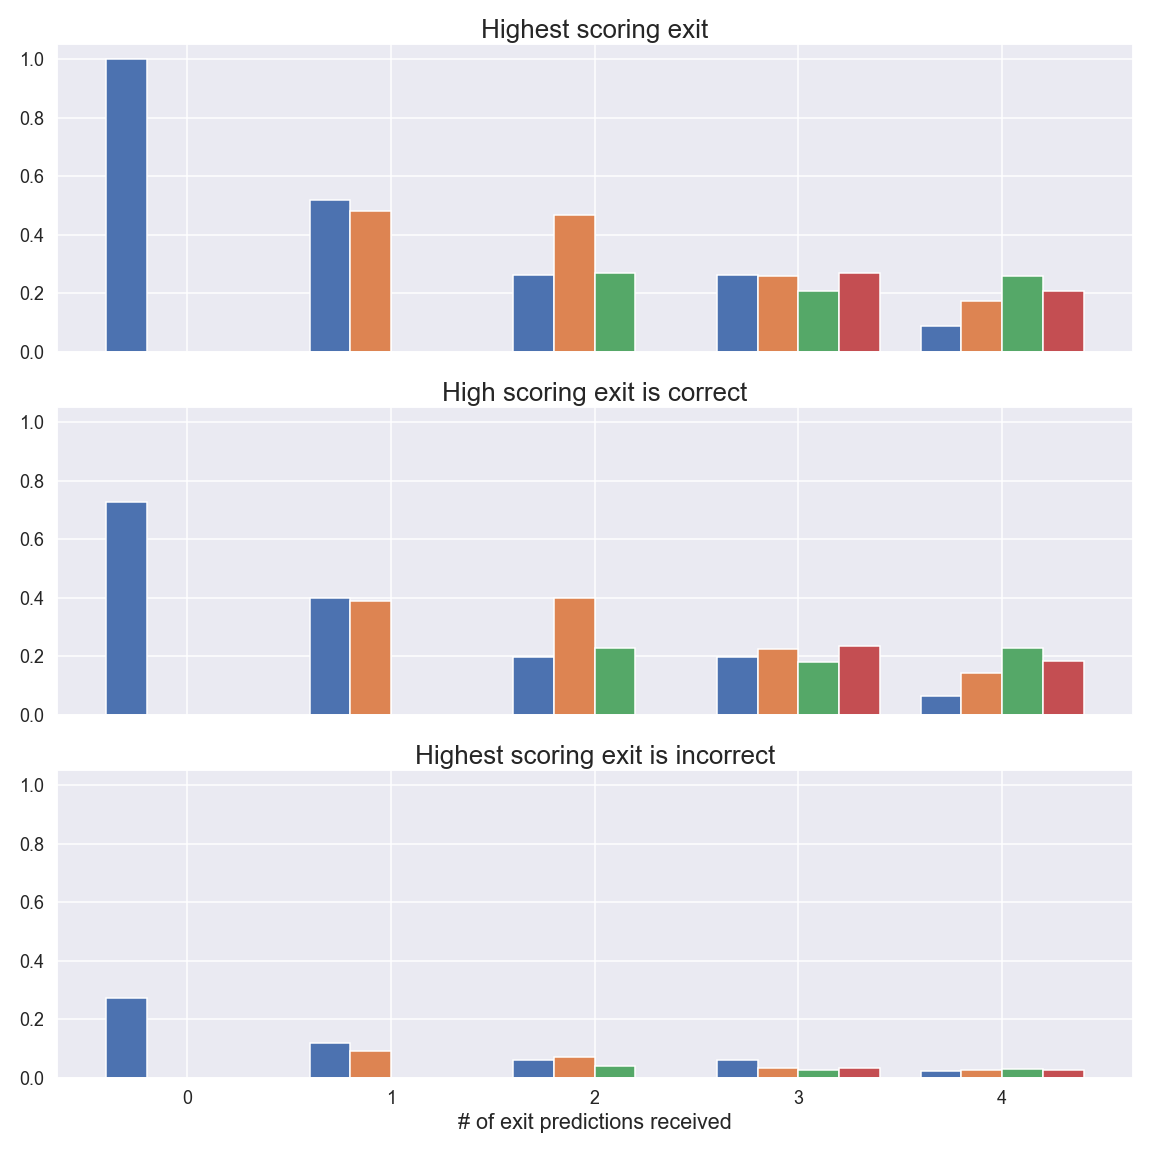
\includegraphics[width=.33\linewidth]{figures/edge/msdnet_correctness}}
	\caption[Highest Scoring Exit]{Highest-scoring exit when one to all predictions are available for \protect\subref{fig:delay-threshold-gpu} \gls{bresnet}, \protect\subref{fig:delay-threshold-jetson} \gls{bdensenet}, and \protect\subref{fig:delay-threshold-nuc} \gls{msdnet} }
	\label{fig:exit-highscore}
\end{figure}

Figure \ref{fig:exit-highscore} shows the distribution of the highest-scoring exit, given the number of exit predictions received. The result shows that the score of later exits is not exclusively higher than the earlier exits. Additionally, it shows whether the highest score exit is correct or incorrect. It shows that the frequency of an early exit being incorrect when it is the highest-scoring is more often than for later exits.

Figure \ref{fig:top-5-cumulative}  shows the top-5 accuracy and cumulative top-5 accuracy. The cumulative top-5 accuracy contains all class labels from the top-5 classes of all previous exits. 
\begin{figure}
	\centering
	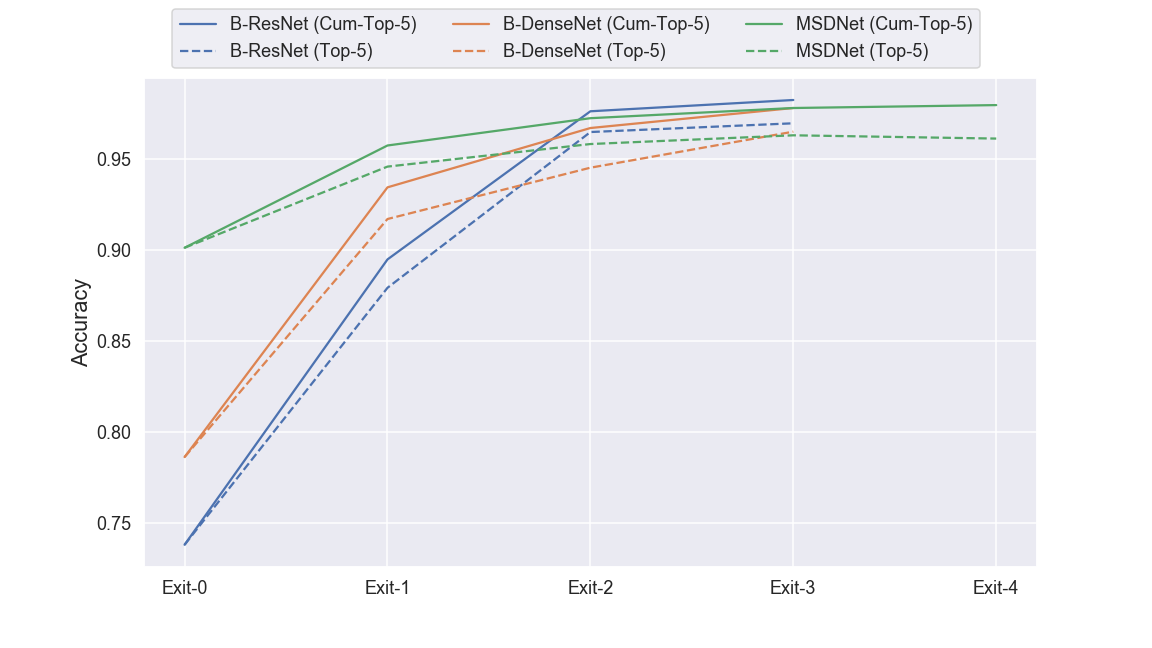
\includegraphics[width=.8\linewidth]{figures/edge/top5cumulative}
	\caption[Top-5 accuracy and Cumulative Top-5 accuracy]{Top-5 accuracy and Cumulative Top-5 accuracy}
	\label{fig:top-5-cumulative}
\end{figure}

The figure shows that having multiple predictions does indeed improve cumulative top-5. Hence there is a better chance of the correct label being in the set of predictions when using all available exit outputs. We question whether we can combine top-5 scores to more confidently select the correct prediction and thereby improve accuracy. 

We analyzed the achievable accuracy using the combination function, having one to all prediction available. In figure \ref{fig:theoretical-info-combi}, we show the results of our analysis.  

The brown line \textit{optimum-top5} would be the maximum achievable accuracy if we were able to cherry-pick the right class among the cumulative top-5 predictions. The purple line \textit{optimum-top1} would be the attainable accuracy if we were able to cherry-pick the correct class among the cumulative top-1 predictions.

Only using the confidence sum for the \gls{msdnet} shows a small improvement in accuracy exclusively when all predictions are available. When predictions from all exits are not available, none of the proposed combination functions can improve the accuracy. There is a more significant difference between the accuracy of the exits of both \gls{bresnet}'s and \gls{bdensenet}'s compared to \gls{msdnet}. The early exit contains more uncertainty, which disturbs the prediction. Furthermore, only the \gls{msdnet} can improve accuracy when having all predictions available.
The score-margin produces the worst results for all models. Thus, having a big difference between the two highest-scoring classes is not equivalent to being correct. Using the  max confidence achieves close to the same performance as using the latest received prediction for \gls{bresnet} and \gls{bdensenet}. Our results show that merely using the latest received predictions is the best overall choice for these early exit models. Henceforth we use the latest received prediction.

\begin{figure}
	\captionsetup[subfigure]{justification=centering,farskip=1pt,captionskip=1pt}
	\centering
	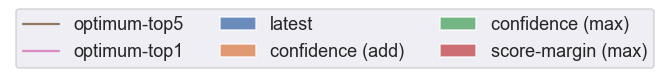
\includegraphics[width=.7\linewidth, keepaspectratio]{figures/edge/theoretical_score_combination_legend}
	\subfloat[B-ResNet\label{fig:combi-resnet}]{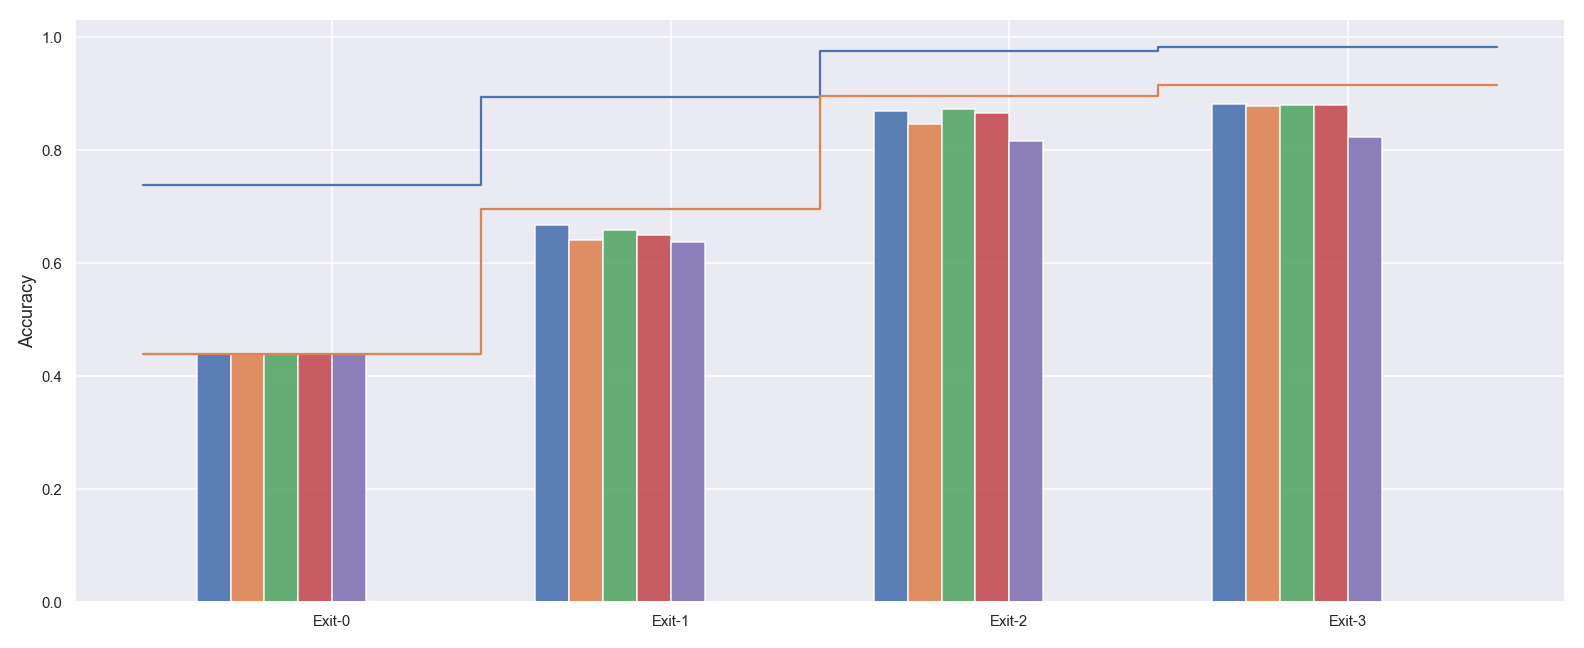
\includegraphics[height=.22\textheight, keepaspectratio]{figures/edge/b-resnet_theoretical_score_combinations}}
	\hfill
	\subfloat[B-DenseNet\label{fig:combi-densenet}]{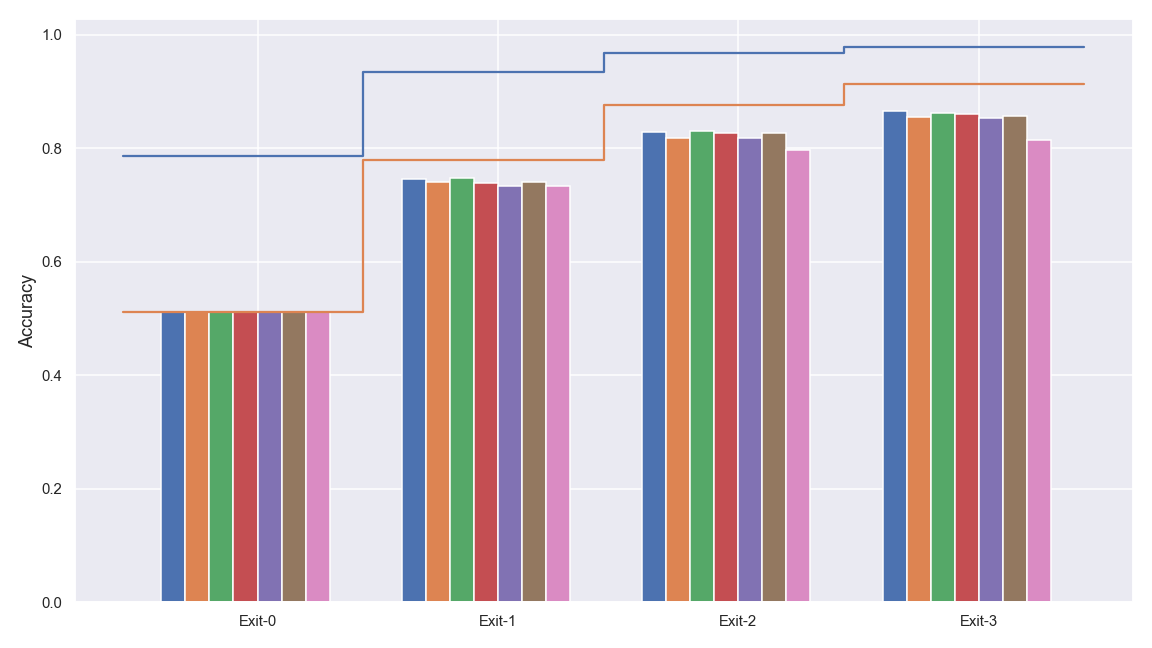
\includegraphics[height=.22\textheight, keepaspectratio]{figures/edge/b-densenet_theoretical_score_combinations}}
	\hfill
	\subfloat[MSDNet\label{fig:combi-msdnet}]{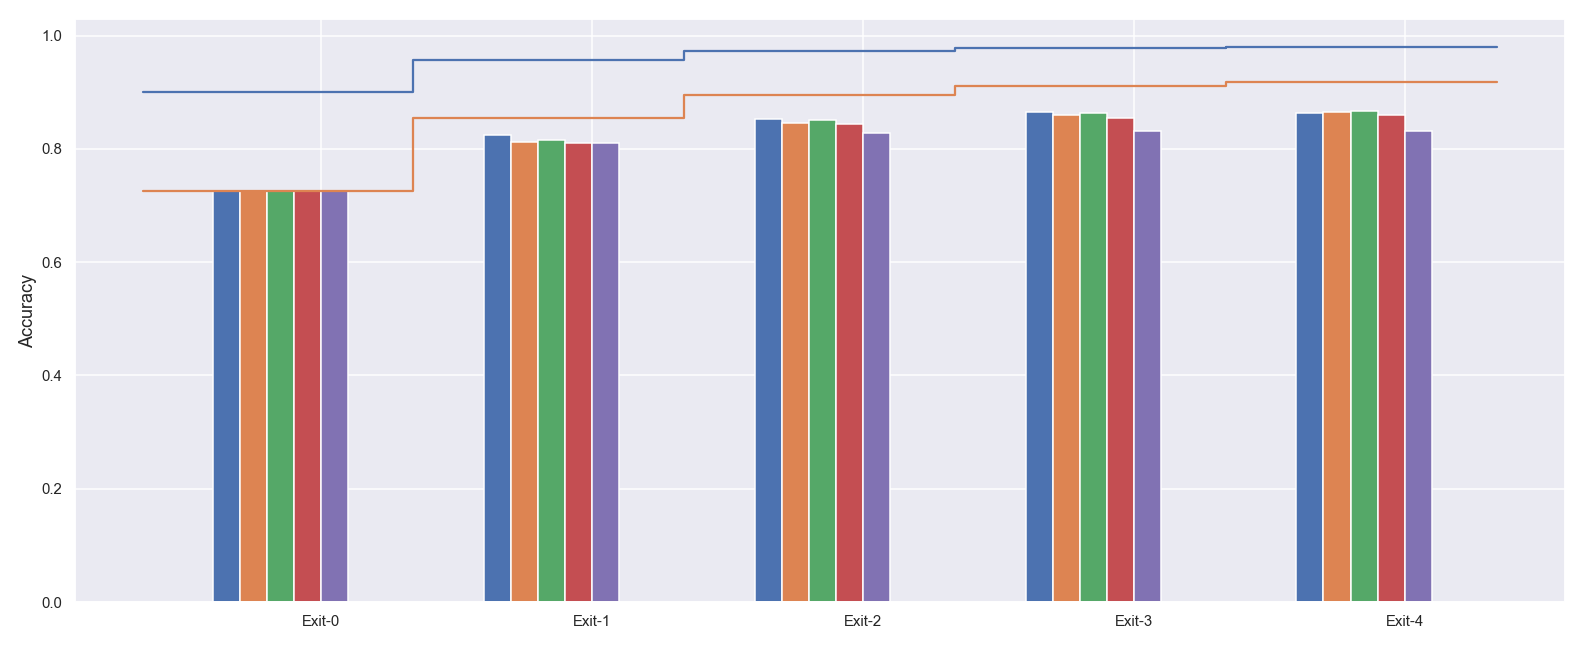
\includegraphics[height=.22\textheight, keepaspectratio]{figures/edge/msdnet_theoretical_score_combinations}}
	\caption[Combination Function with $ n $ Available Exits]{Combination Function with $ n $ Available Exits for \protect\subref{fig:combi-resnet} \gls{bresnet}, \protect\subref{fig:combi-densenet} \gls{bdensenet}, and \protect\subref{fig:combi-msdnet} \gls{msdnet}}
	\label{fig:theoretical-info-combi}
\end{figure}


\subsection{Edge Offloading: \gls{aee} vs. Conventional Offloading}

We set up our implementation using NUC as an end-device and both \gls{jetson} and \gls{gpu-ws} as edge servers. We let all the inference of validation samples be offloaded to the edge servers. For the delay threshold we use 0.1ms granularity by setting $\delta = \{0.1,0.2, \dots, 250.0\}$. Figure \ref{fig:practical-offloading} shows the achieved reliability for the delay threshold. 

\begin{figure}
	\captionsetup[subfigure]{justification=centering,farskip=1pt,captionskip=1pt}
	\centering
	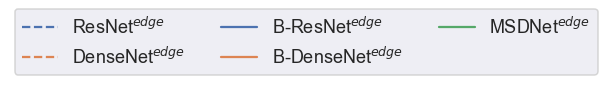
\includegraphics[width=.5\linewidth]{figures/edge/offloading_legend}
	\subfloat[\gls{jetson}\label{fig:offloading-jetson}]{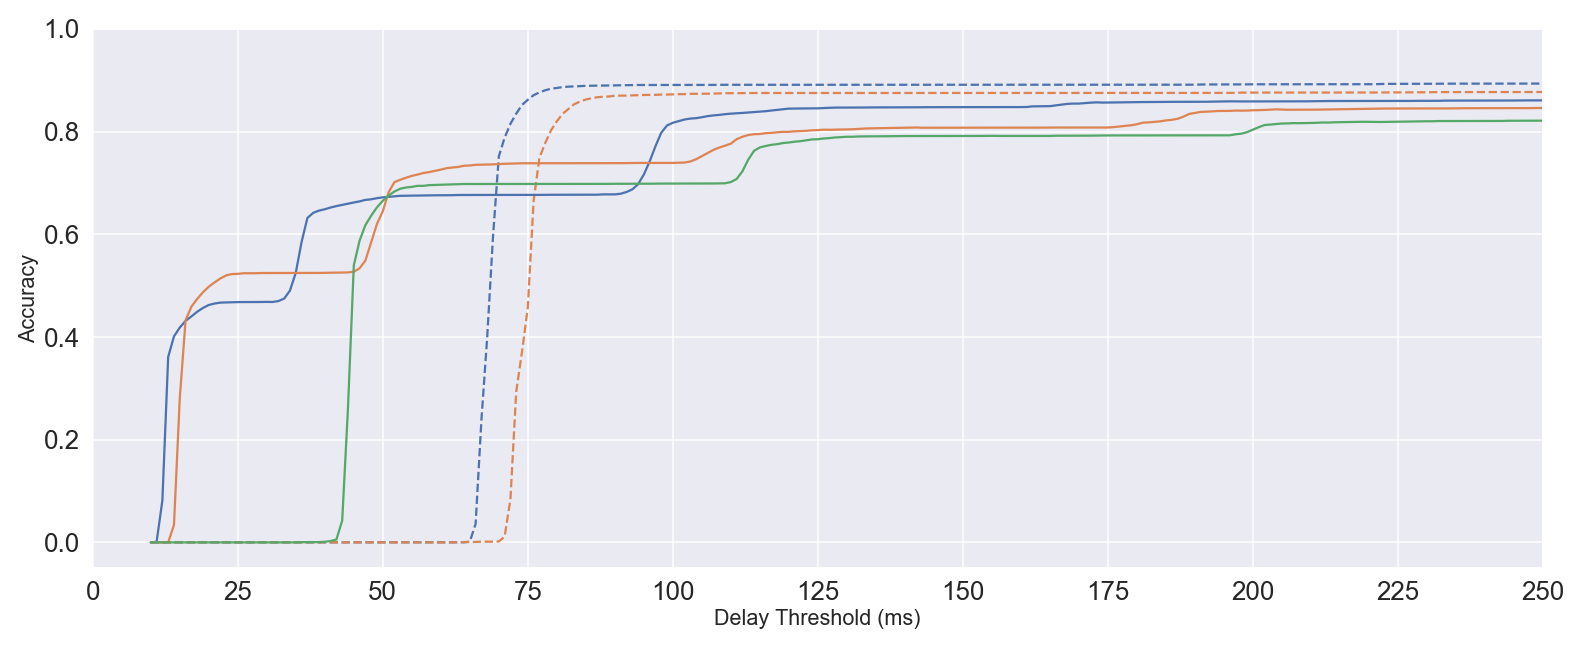
\includegraphics[width=.8\linewidth]{figures/edge/jetson_offloading}}
	\hfill
	\subfloat[\gls{gpu-ws}\label{fig:offloading-gpu}]{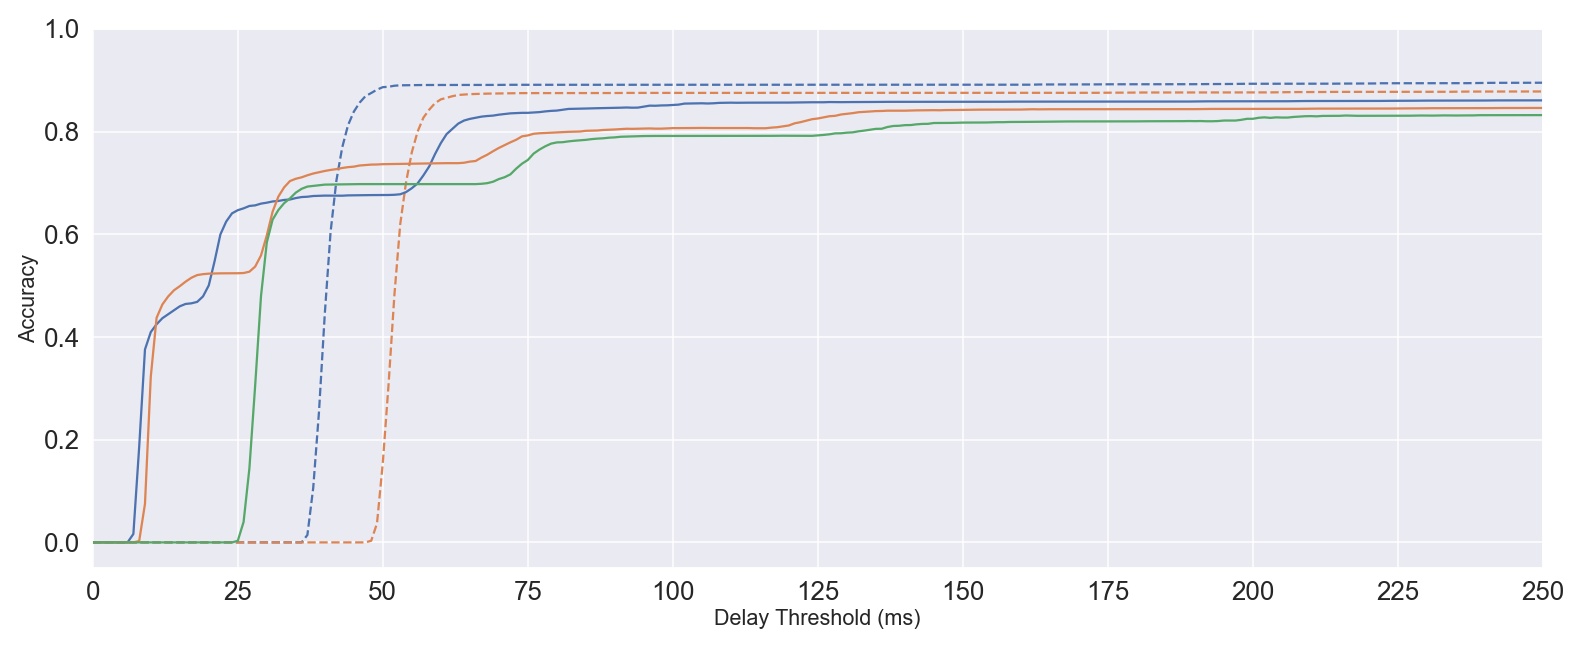
\includegraphics[width=.8\linewidth]{figures/edge/gpu_offloading}}
	%	\subfloat[Local Jetson TX2]{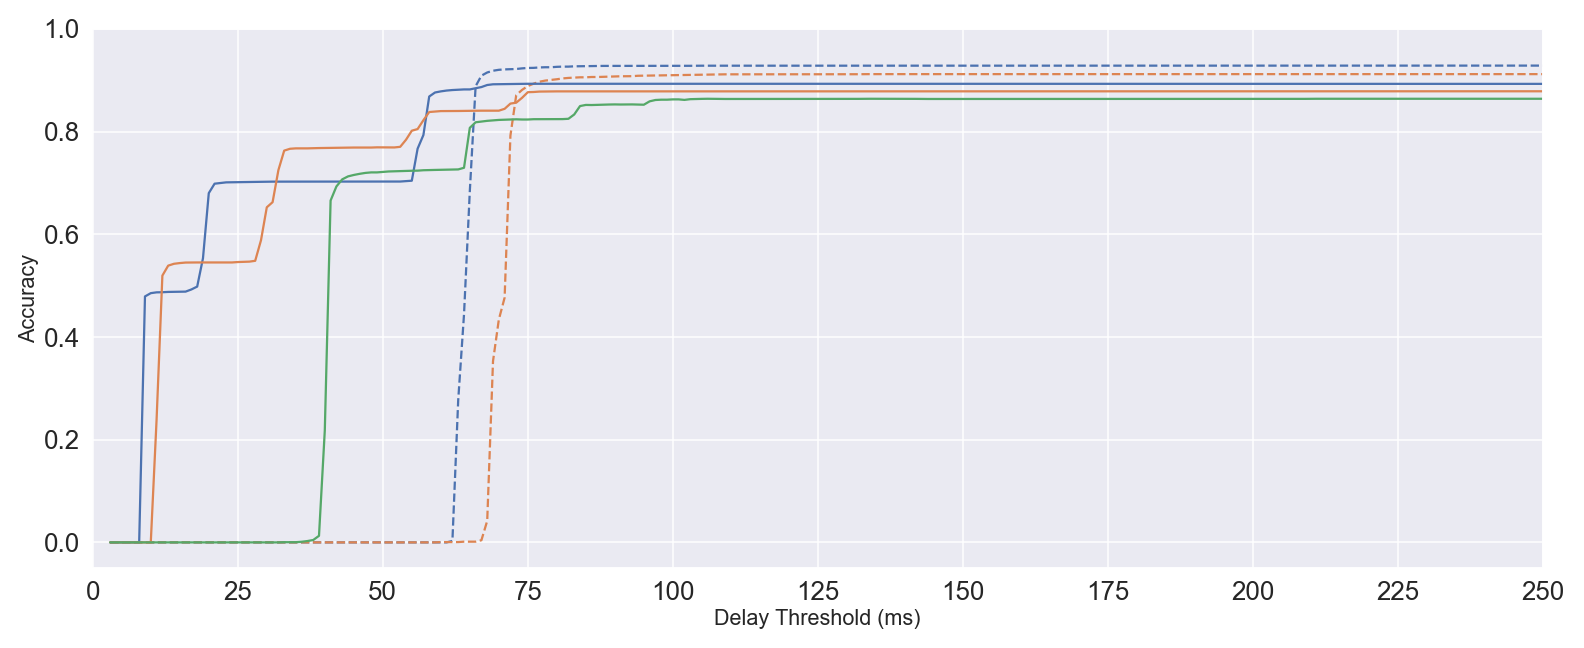
\includegraphics[width=\linewidth]{figures/delay_plots/jetson__delay_threshold}}
	\caption[Offloading Reliability]{Offloading reliability vs. delay threshold from NUC to \protect\subref{fig:offloading-jetson} \gls{jetson}, and \protect\subref{fig:offloading-gpu} \gls{gpu-ws}.}
	\label{fig:practical-offloading}
\end{figure}

Generally, the \gls{gpu-ws} achieves higher reliability at lower delays than the \gls{jetson}. The figure shows how \gls{aee} enables service at more stringent delay thresholds that are not even possible when offloading conventional models for edge inference. The scheme successfully improves the reliability below 75 ms for the \gls{jetson}, and below 50 ms for the \gls{gpu-ws} using \gls{bresnet} and \gls{bdensenet}. 
No model achieves superior reliability at all delays, which means the selection of models should be based on the delay threshold, the available bandwidth, and the inference latency. The figure shows the model to select given the delay threshold with the available bandwidth for this test by selecting the model, achieving the highest reliability.

\subsection{Local On-Device Inference vs. Edge Offloading}

We compare edge offloading inference to edge servers with local inference on the \gls{nuc}. In figure \ref{fig:resnet-offloading-vs-local}, we compare the \gls{resnet}-based models. In figure \ref{fig:densenet-offloading-vs-local}, the \gls{densenet}-based models, and lastly, in figure \ref{fig:msdnet-offloading-vs-local}, the \gls{msdnet} model.
Generally, the figures show the impact of adding communication. Communication latency introduces additional uncertainty, which softens the curves and makes the steps to next exit less sharp compared to local inference. Note, there is a gap in reliability between local and edge. The reason why local execution can obtain higher reliability is due to deadline violations caused by significant variations in communication time. If we extend the x-axis to go above 1s, we would be able to see that the gap is closing. 
\begin{figure}
	\captionsetup[subfigure]{justification=centering, farskip=0pt,captionskip=0pt}
	\centering
	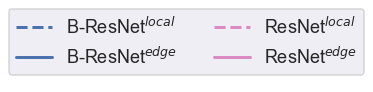
\includegraphics[width=.3\linewidth]{figures/edge/gpu_b-resnet_offloading_vs_local_legend}
	\hfill
	\subfloat[\gls{jetson} as Edge\label{fig:resnet-offloading-vs-local-jetson}]{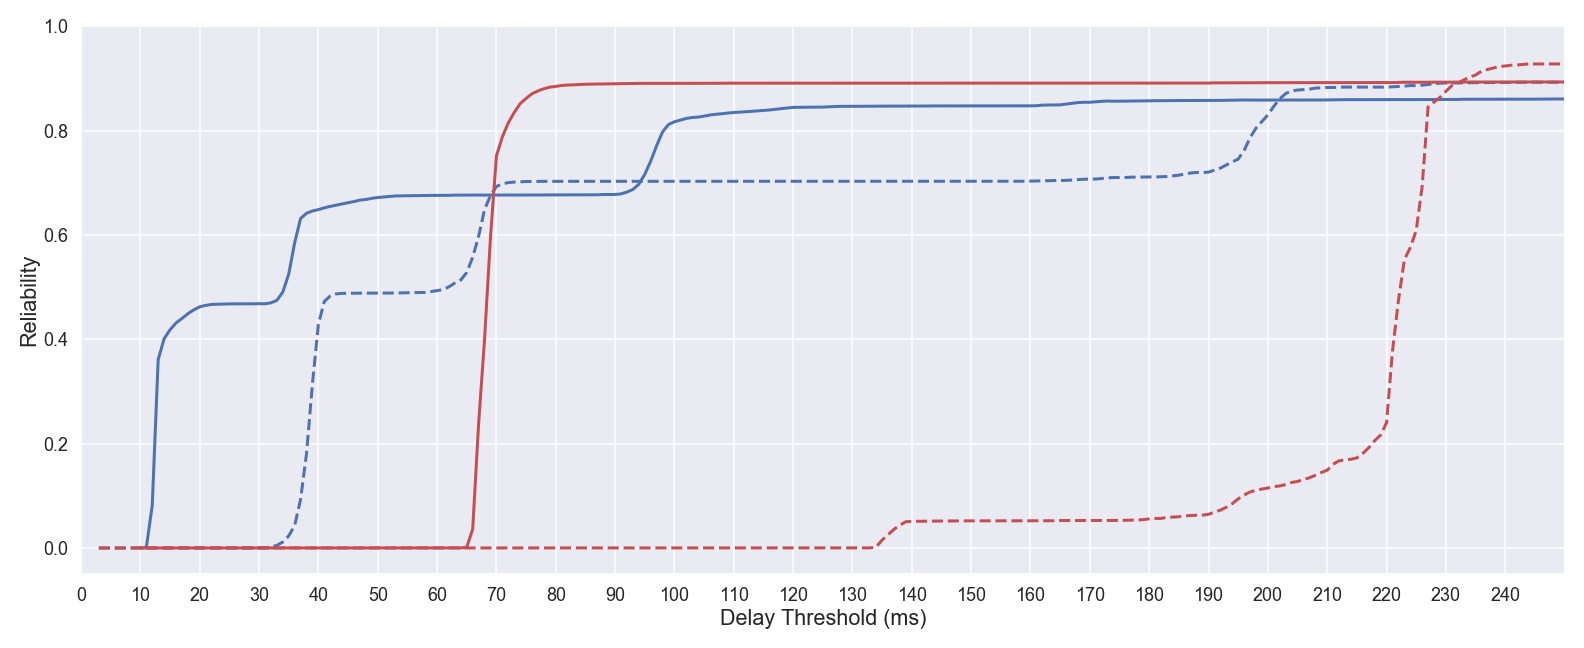
\includegraphics[width=\textwidth,height=.22\textheight,keepaspectratio]{figures/edge/jetson_b-resnet_offloading_vs_local}}
	\hfill
	\subfloat[\gls{gpu-ws} as Edge\label{fig:resnet-offloading-vs-local-gpu}]{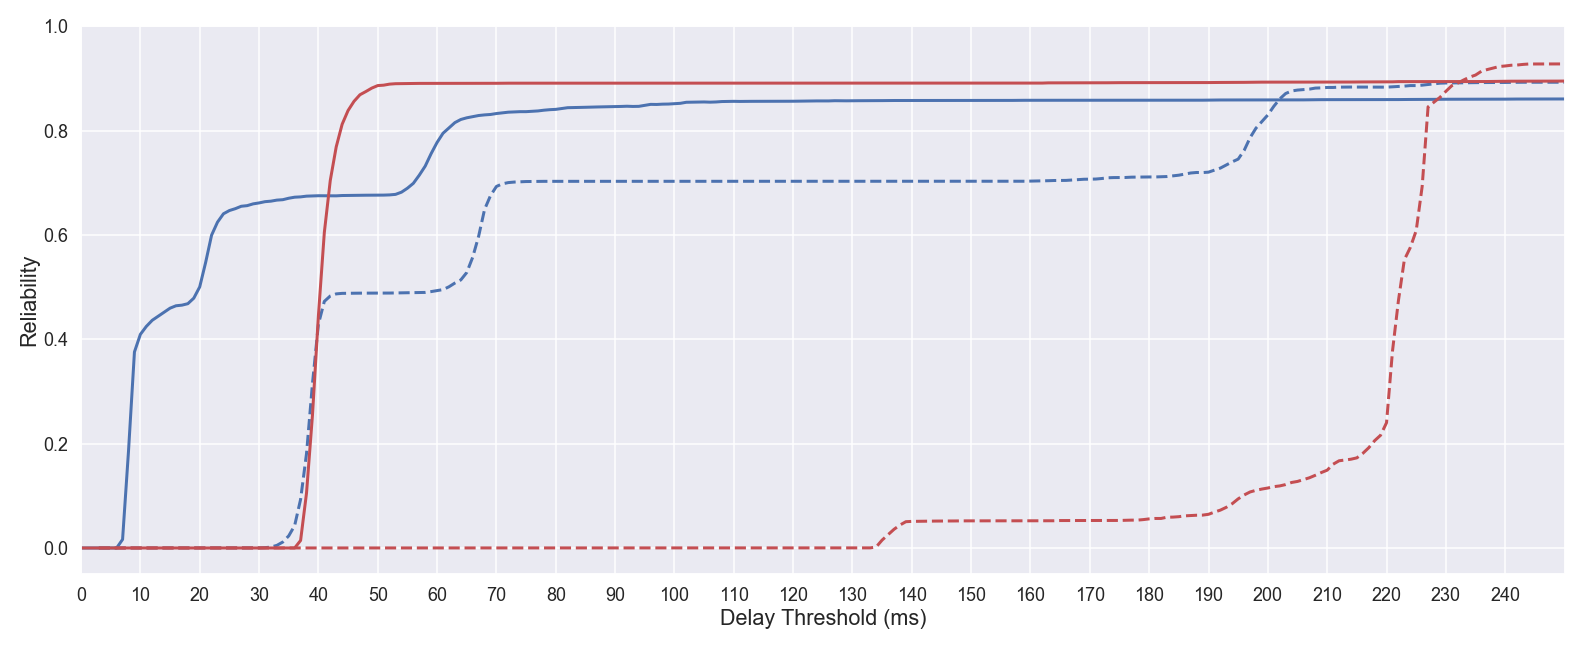
\includegraphics[width=\textwidth,height=.22\textheight,keepaspectratio]{figures/edge/gpu_b-resnet_offloading_vs_local}}
	\caption[Offloading comparison of residual networks]{Reliability vs. delay threshold for local inference and offloaded \gls{aee} compared with conventional schemes for the residual networks.}
	\label{fig:resnet-offloading-vs-local}
\end{figure}

Figure \ref{fig:resnet-offloading-vs-local} shows how the \gls{aee} scheme for edge offloading can improve the reliability under stringent delay requirement using either platform as edge server instead of local inference. Also, it improves the reliability compared to using a conventional model again under stringent requirements. When offloading, the conventional model starts to outperform the early exit model if we allow 80 ms runtime using the Jetson TX2 or 50ms runtime using the GPU Workstation. The local inference would be the best option if the application can tolerate 250ms delay. However, the time-critical IoT applications require much shorter delays. 
\begin{figure}
	\captionsetup[subfigure]{justification=centering, farskip=0pt,captionskip=0pt}
	\centering
	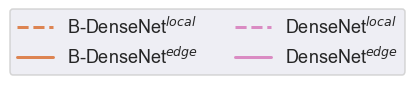
\includegraphics[width=.3\linewidth]{figures/edge/gpu_b-densenet_offloading_vs_local_legend}
	\hfill
	\subfloat[\gls{jetson} as Edge\label{fig:densenet-offloading-vs-local-jetson}]{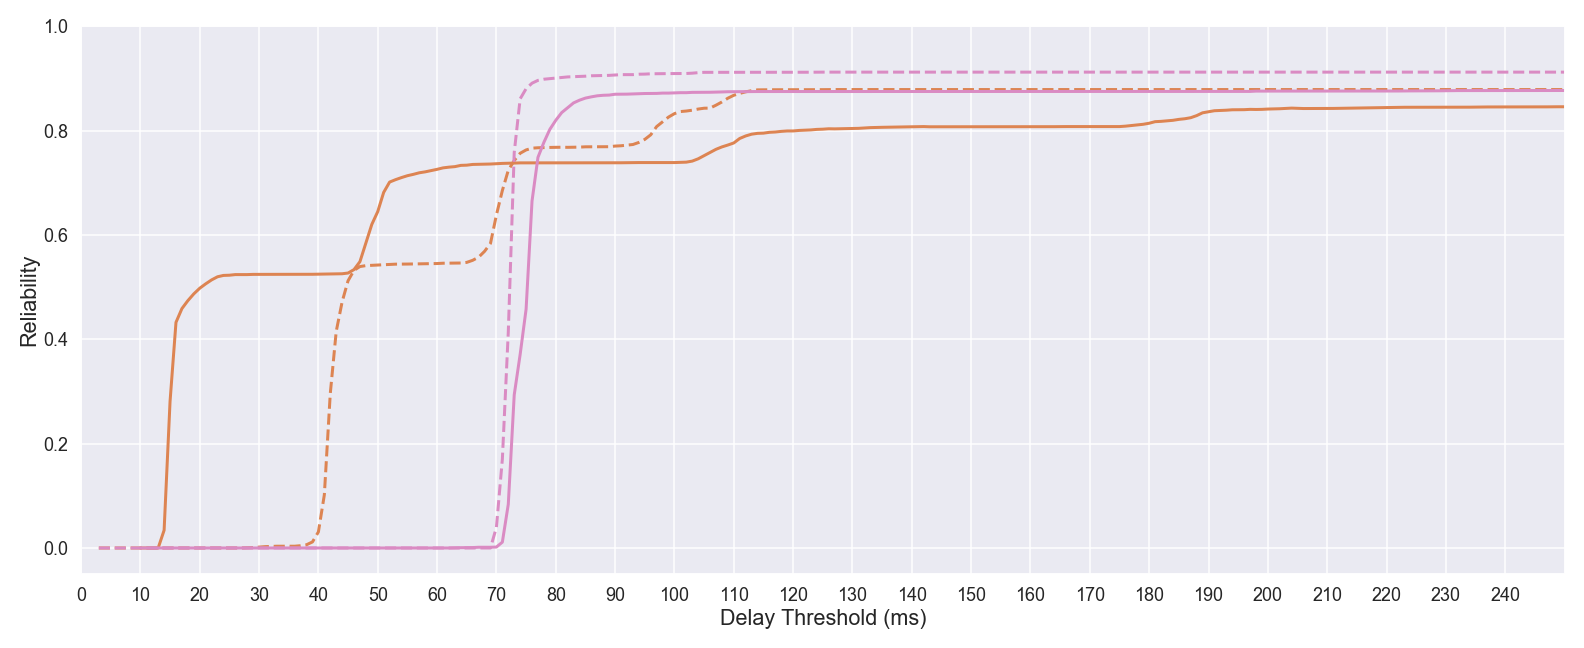
\includegraphics[width=\textwidth,height=.22\textheight,keepaspectratio]{figures/edge/jetson_b-densenet_offloading_vs_local}}
	\hfill
	\subfloat[GPU Workstation as Edge\label{fig:densenet-offloading-vs-local-gpu}]{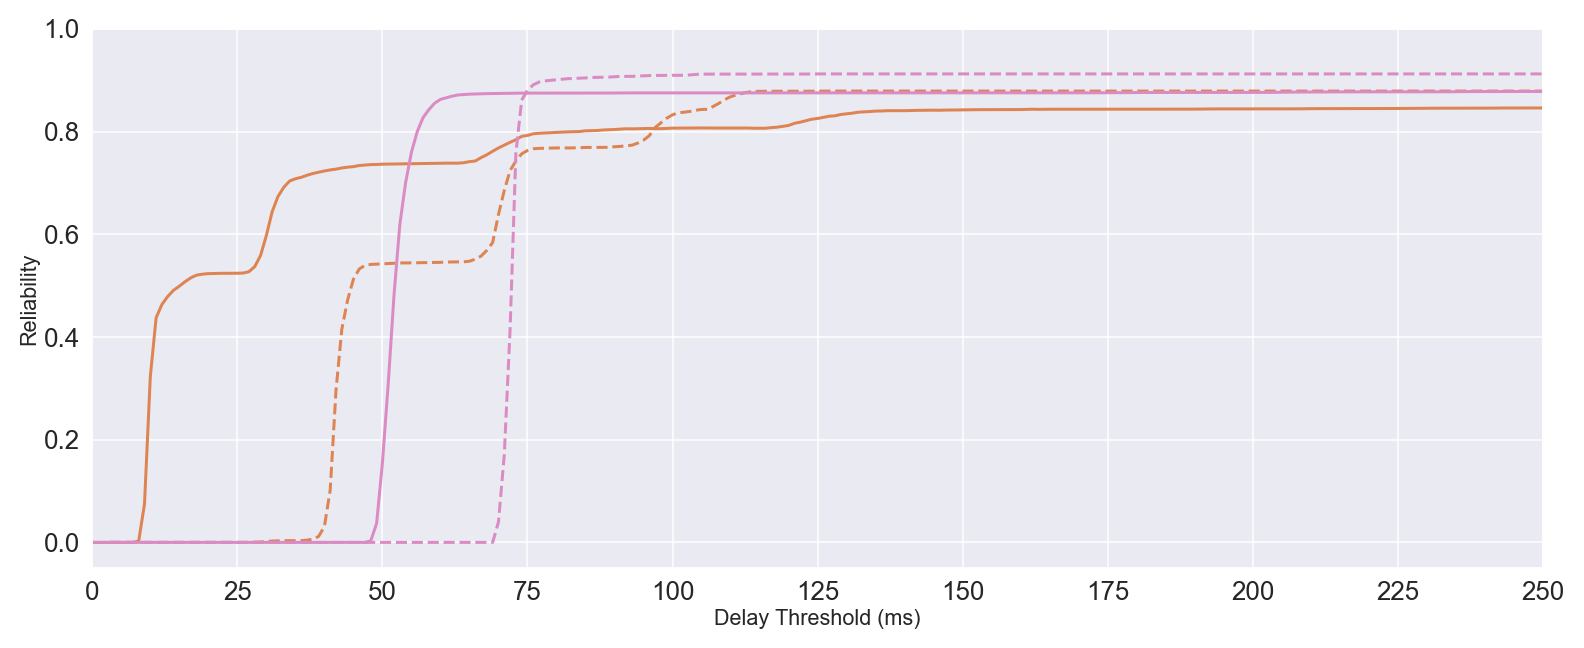
\includegraphics[width=\textwidth,height=.22\textheight,keepaspectratio]{figures/edge/gpu_b-densenet_offloading_vs_local}}
	\caption[Offloading comparison of densely connected networks]{Reliability vs. delay threshold for local inference and offloaded \gls{aee} compared with conventional schemes for the densely connected networks.}
	\label{fig:densenet-offloading-vs-local}
\end{figure}

The \gls{densenet}s tell a somewhat different story. We are still able to improve reliability significantly under stringent delay requirements using \gls{aee} compared to offloading a conventional model and also to local inference. However, when reaching 70-80 ms on \gls{jetson}, all other schemes start to outperform  \gls{aee} edge offloading. Note that local inference of the conventional model is always faster than offloading to \gls{jetson}. For the \gls{gpu-ws} offloading, the conventional model is more reliable under 75 ms. We can conclude that the difference in computing performance between the \gls{jetson} and \gls{nuc} is small. The \gls{nuc} is a relatively powerful device compared to other \gls{iot} devices, e.g., the Raspberry Pi. The \gls{nuc} has a low power Intel i7 \gls{cpu}. In most scenarios in real-life, end-devices are more likely to be equipped with low-end ARM processors or even smaller processing units, which will degrade the inference time of any of the models. In \cite{zheng_apache/incubator-tvm_nodate}, they report an average runtime of 726.0 ms of \gls{resnet}50 on Raspberry Pi, i.e., such low-end devices are infeasible for real-time processing. Other end-devices may not even be able to run any of the models locally, which makes offloading inevitable. Given these results, the edge servers may not necessarily need to be equipped with powerful \gls{gpu}s, as the NUC can achieve such high performance, especially when running the \gls{msdnet}. 

\begin{figure}
	\captionsetup[subfigure]{justification=centering, farskip=0pt,captionskip=0pt}
	\centering
	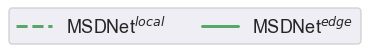
\includegraphics[width=.3\linewidth]{figures/edge/gpu_msdnet_offloading_vs_local_legend}
	\hfill
	\subfloat[\gls{jetson} as Edge]{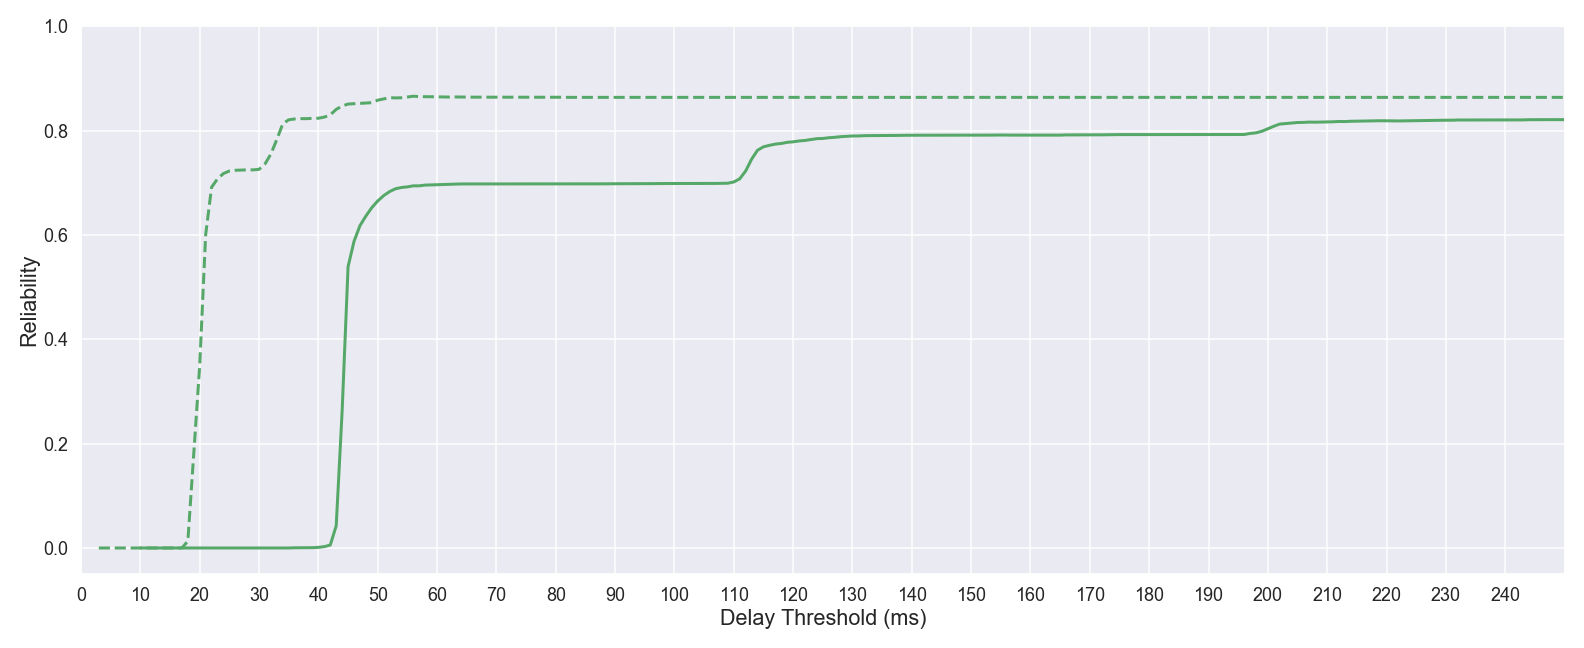
\includegraphics[width=\textwidth,height=.22\textheight,keepaspectratio]{figures/edge/jetson_msdnet_offloading_vs_local}}
	\hfill
	\subfloat[\gls{gpu-ws} as Edge]{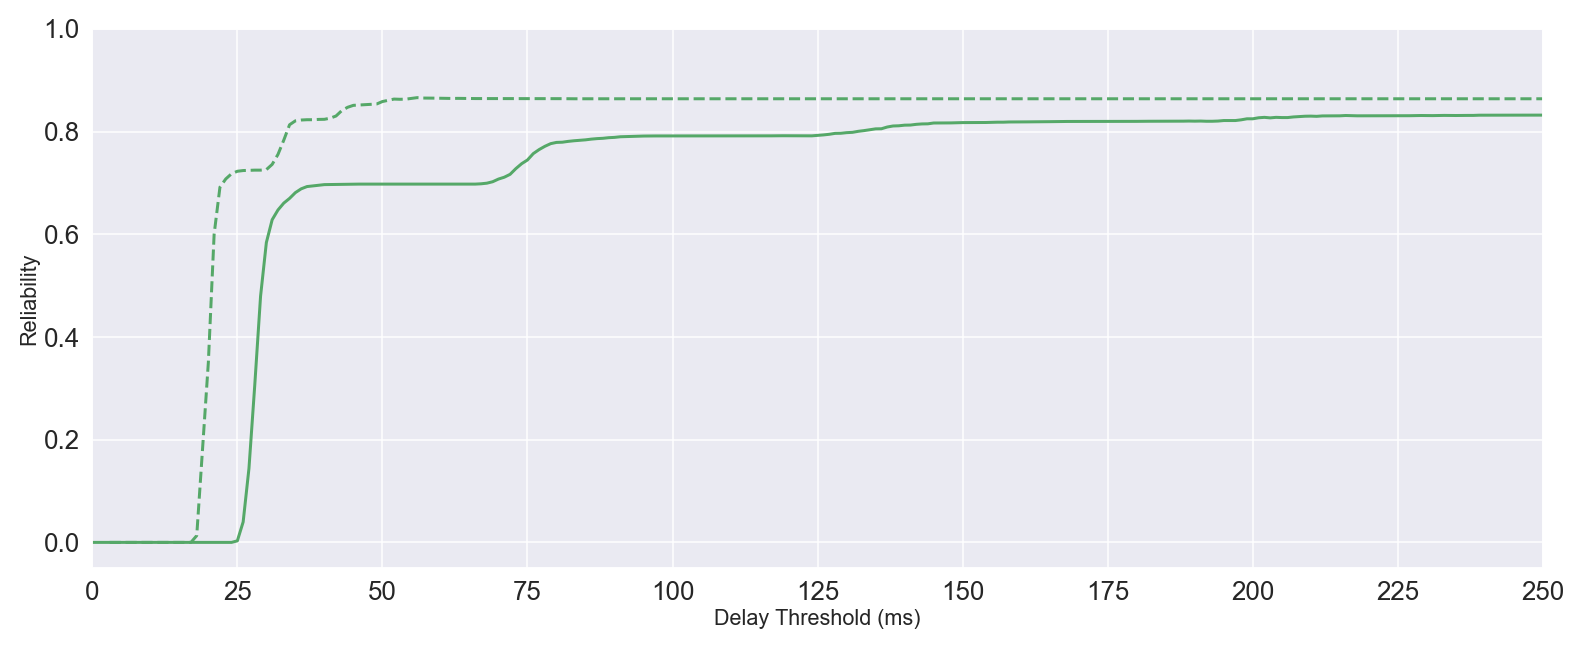
\includegraphics[width=\textwidth,height=.22\textheight,keepaspectratio]{figures/edge/gpu_msdnet_offloading_vs_local}}
	\caption[Offloading comparison of multi-scale dense networks]{Reliability vs. delay threshold for local inference and offloaded \gls{aee} compared with conventional schemes for the multi-scale dense networks.}
	\label{fig:msdnet-offloading-vs-local}
\end{figure}

The \gls{msdnet} tells an entirely different story. The local inference is always able to achieve higher reliability, disregardless of offloading to \gls{jetson} or \gls{gpu-ws}. 

In general, offloading \gls{aee} to the edge improves system reliability compared to on-device \gls{aee} inference. Especially, \gls{aee} using \gls{bresnet} at the edge outperforms the local inference of the \gls{resnet}-based model under stringent latency requirements. The improvement is most significant when using the \gls{gpu-ws}, which is a significantly more powerful machine. For the \gls{msdnet}, our offloading solution was uncompetitive with local execution. These results illustrate the complexity of offloading the inference task, as we were not able to find a single model that provided the best reliability for all delay thresholds.

\subsection{Communication Latency}

We measured the communication times for offloading. In table \ref{tbl:time-offloading},
we present the statistics for the measurements.
\begin{longtabu}{>{\bfseries}X[2]|X|X|X|X}
	\caption[Communication Statistics]{Communication Statistics} \label{tbl:time-offloading} \\
	\toprule
	\rowfont{\bfseries} & Mean (ms) & Std. (ms) & Min (ms) & Max (ms) \tabularnewline
	\bottomrule
	\endfirsthead
	\multicolumn{3}{@{}l}{\textbf{\textcolor{black}{Table \ref{tbl:time-offloading}:}} continued}\\
	\toprule
	\rowfont{\bfseries} & Mean (ms) & Std. (ms) & Min (ms) & Max (ms) \tabularnewline
	\bottomrule
	\endhead % all the lines above this will be repeated on every page
	\bottomrule
	\multicolumn{3}{@{}l}{continued \ldots}\\
	\endfoot
	\hline
	\endlastfoot
	Communication time	& 25.68	& 110.93 & 2.35 & 962.76  \tabularnewline						
	\bottomrule
\end{longtabu}

The meantime for the communication delay was 25ms, with a standard deviation of 110.93ms, which exemplifies the instability of communication delays. In the worst case, it takes almost 1s to send an image.

To examine the impact of reliable communication, we set up another test. The images are sent from the client to the server. Using \gls{wireshark} \cite{noauthor_wireshark_nodate}, we logged the network traffic and analyzed the package overhead, e.g., acknowledgments packets, retransmission packets, and other controlling overhead used by \gls{tcp} to ensure reliable transmission. Figure \ref{fig:tcp-overhead} shows the density of \gls{tcp} package overhead for three scenarios. 
\begin{figure}
	\centering
	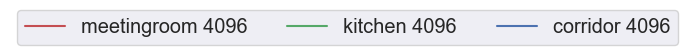
\includegraphics[width=.5\linewidth]{figures/tcp/density_legend}
	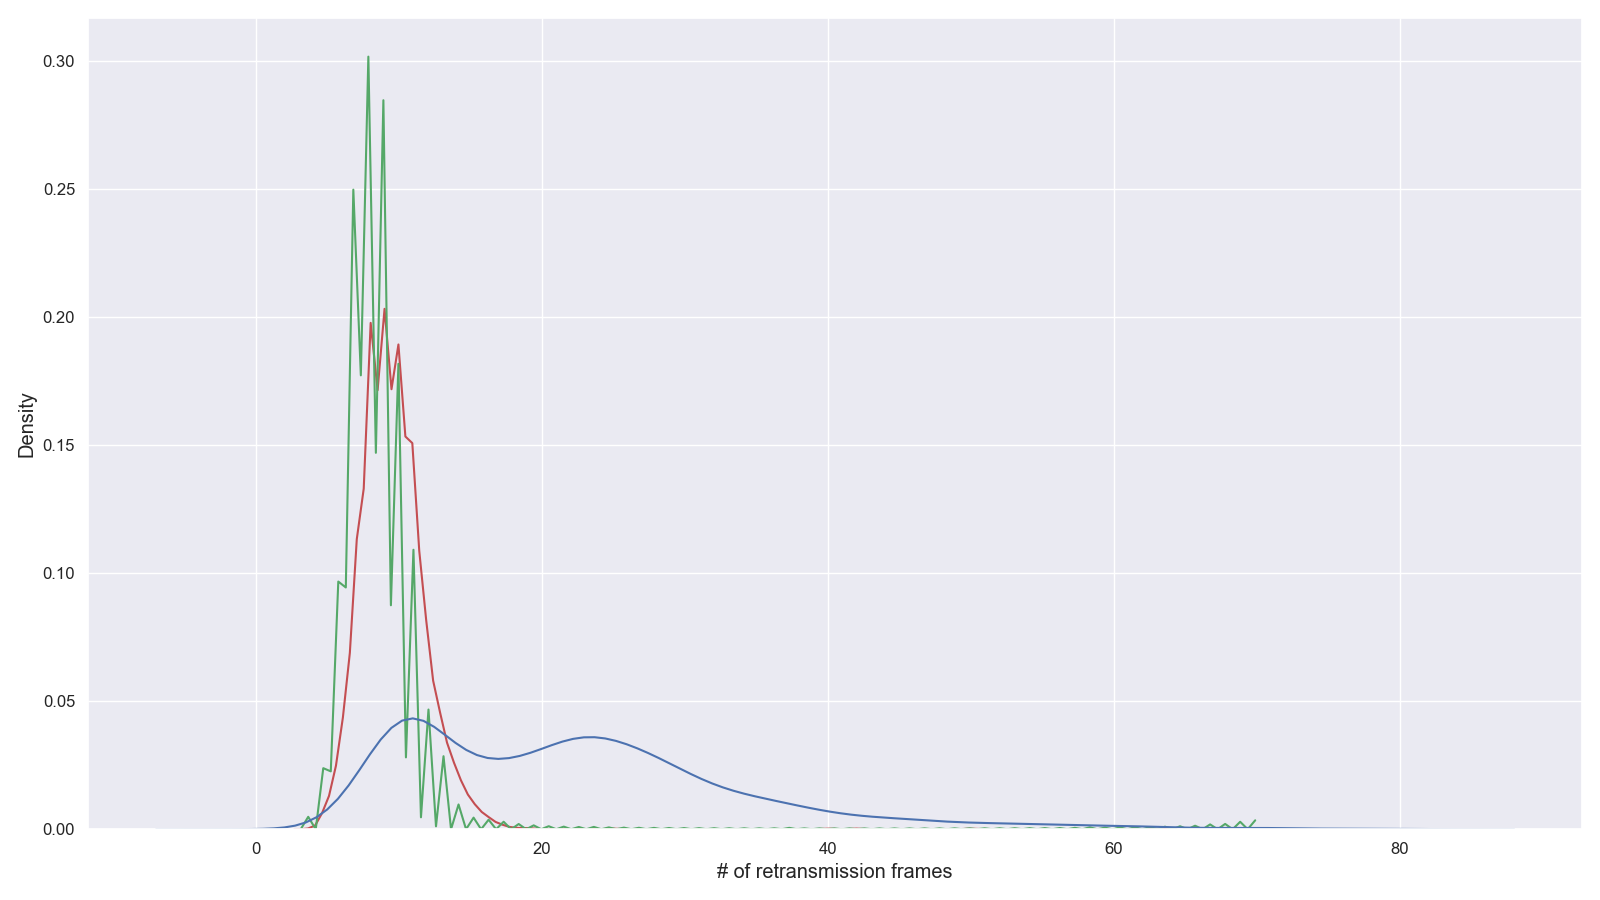
\includegraphics[width=.7\linewidth]{figures/tcp/density}
	\caption[TCP retransmission overhead]{TCP packet overhead}
	\label{fig:tcp-overhead}
\end{figure}
The test was made in three different scenarios (meeting room, kitchen, and corridor). For the scenarios, the end-device is moved further away from the server. The distance reduces the quality of the communication link. In a poor communication environment, \gls{tcp} can be expected to have a high overhead caused by increasing packet overhead, from particularly retransmissions, thus harming the overall delay.  

\section{Summary} \label{sec:edge-summary}

We examined the combination functions for the client-side selection of the prediction.  We did not find a combination function that improved accuracy.  The best option is to use the lastest received prediction within the time frame

Using \gls{aee} for edge offloading enables service at more stringent delay thresholds not even possible when offloading conventional models for edge inference. The scheme successfully improves the reliability below 75 ms for the \gls{jetson}, and below 50 ms for the \gls{gpu-ws} using \gls{bresnet} and \gls{bdensenet}. Offloading the different models show overlapping reliability of the \gls{bresnet} and \gls{bdensenet}, hence it depends on the delay threshold which model to select.

Generally, offloading \gls{aee} improves reliability compared to the local inference of \gls{aee}. When offloading to the powerful server, i.e., for the \gls{gpu-ws}, the reliability for \gls{bresnet} is improved for delays below 200ms and 100ms for the \gls{densenet}. With the \gls{jetson} as edge, the reliability of both \gls{bresnet} and \gls{bdensenet} is improved below 70ms. Neither server could achieve competitive reliability to the local inference of the \gls{msdnet}.

We investigate the impact of reliable communication and show large variations in delay when introducing communication. \gls{tcp} can cause long delays in a poor communication environment, which harms the reliability of real-time service. In chapter \ref{ch:discussion}, we discuss alternatives to \gls{tcp}.




